\documentclass[12pt,a4paper,article]{bpm2}

\usepackage{NiOMGTU}

\usepackage{cmap}
\usepackage[utf8x]{inputenc}
\usepackage[T2A]{fontenc}
\usepackage[english,russian]{babel}

\title{Выбор функции распределения состояний\\при параллельной проверке модели}
\author{И.\,А.\,~Коротков, В.\,А\,.~Крищенко}
\UDK{004.021}
\email{kva@bmstu.ru}    %  список через запятую, символ _ набирается как \_

\IssCode{??????}       %  код выпуска
\issue{?}              %  номер выпуска
\issuemonth{12}         %  месяц выпуска
\issueyear{2011}       %  год выпуска
\htmlname{??????}

\usepackage{graphicx}

\def\baselinestretch{1.2}

\begin{document}

\maketitle

\section-{Введение}

Проверка модели (model checking)~--- автоматический формальный подход, при котором на основе конечной дискретной модели программы или комплекса программ строится полное пространство состояний и на нем проверяется набор интересующих нас утверждений~--- спецификация~\cite{Clarke}.
Основной проблемой данного метода является <<комбинаторный взрыв>> числа состояний при росте размера модели и, как следствие, невозможность хранить пространство состояний целиком в доступной памяти.

В настоящий момент на практике применяется ряд оптимизаций, позволяющих сократить как число состояний, так и требуемый для их хранения объем ОЗУ: сокращение частных порядков~\cite{Clarke}, битовое хэширование без обнаружения коллизий~\cite{BitHash1}, сжатие состояний.
Однако, данные меры либо дают небольшой, плохо масштабируемый прирост, либо приводят к потенциальным потерям состояний при обходе.
Альтернативным подходом является параллельная генерация состояний с распределенным хранением по различным узлам вычислительного кластера.
При этом от выбора функции распределения состояний между узлами зависит число удаленных вызовов между узлами и общее время проверки модели.

Статья организована следующим образом. В разд.~\ref{sec:modelchecking} дано формальное определение модели и проверяемой спецификации. В разд.~\ref{sec:spin} приведены описание языка Promela и пример модели, заданной с его помощью. В разд.~\ref{sec:pargen} описан общий алгоритм параллельной генерации состояний, а в разд.~\ref{sec:state-partition} приведена предлагаемая функции разбиения пространства состояний. Наконец, в разд.~\ref{sec:implementation} описан используемый для экспериментов прототип, а в разд.~\ref{sec:experim} представлены результаты экспериментов.

\section{Проверка конечных моделей}
\label{sec:modelchecking}

Пространство состояний детерминированной системы, например, моделируемой программы, можно формализовать в виде модели Крипке~\cite{Clarke}.
Моделью Крипке $M$ над множеством атомарных высказываний $AP$
называют четверку $(S, S_0, R, L)$, где:

\begin{itemize}
\item $S$~--- конечное множество состояний;
\item $S_0 \in S$~--- множество начальных состояний;
\item $R \in S \times S$~--- отношение переходов, которые обязано быть тотальным, т.е. для каждого состояния $s \in S$
  должно существовать такое состояние $s' \in S$, что имеет место $R(s, s')$;
\item $L\colon S \rightarrow 2^{AP}$~--- функция, которая помечает каждое состояние множеством  атомарных высказываний, истинных в этом состоянии.
\end{itemize}

Путь в модели $M$ из состояния $s$~--- это бесконечная последовательность состояний $\pi = s_0 s_1 \ldots$, такая, что
$s_o = s$ и для всех $i \geq 0$ выполняется $R(s_i, s_{i+1})$.

Моделируемая программа в каждом своем состоянии описывается набором значений переменных $V = \{v_0, v_1, \ldots\}$, принимающих значения на конечном множестве $D$ (домене интерпретации) и описывающих отдельные компоненты модели и взаимодействие между ними.
Множество $AP$ состоит из утверждений вида $v_i = d_i$, где $d_i \in D$.
Таким образом, каждое состояние $s$ в $M$ представляет собой отображение $V \rightarrow D$.

Отношение $R$ определяется следующим образом. Пусть имеются два состояния, $s_1$ и $s_2$. Если в $s_1$ имеется
компонент, который может выполнить атомарный переход (изменение значений своих переменных), в результате выполнения
которого система будет находиться в состоянии $s_2$, тогда состояния $s_1$ и $s_2$ связаны отношением перехода: $(s_1,
s_2) \in R$. В случае, если нет такого состояния $s_2$, для которого бы выполнялось $R(s_1, s_2)$, полагается $R(s_1,
s_1)$, т.е. <<тупиковое>> состояние связано отношение перехода само с собой.

Для формализации проверяемых на модели $M$ утверждений обычно используются временные логики~\cite{Clarke}.
Однако, для проверки моделей программных систем наиболее актуальны два вида высказываний:
\begin{itemize}
\item утверждение о постоянном выполнении некоего условия в заданной точке компонента, что является аналогом конструкции \textbf{assert} при программировании;
\item утверждение о завершении работы модели или её функционировании в вечном цикле, что важно при поиске тупиков в программной системе.
\end{itemize}

\section{Язык описания модели}
\label{sec:spin}

Наиболее распространенным средством проверки конечных моделей является система SPIN, использующее для описания исходной
модели язык Promela~\cite{SPIN}.

Модель на языке Promela описывается в виде набора процессов (компонент модели), состоящих из последовательности команд.
Каждый процесс имеет свой набор локальных переменных, в том числе счетчик команд.
Для взаимодействия между процессами могут использоваться глобальные переменные и очереди сообщений.
Каждая команда имеет свое условие выполнимости, и процесс считается заблокированным, если условие выполнимости его текущей команды не выполнено.

Пример описания модели семафора Дейкстры и трех захватывающих его процессов в нотации языка Promela приведен ниже.
Для данной модели представляет интерес утверждение о «вечном» выполнении модели, что будет свидетельствовать об отсутствии тупиков.

{\small
\begin{verbatim}
mtype { p, v };
chan sema = [0] of { mtype };
active proctype dijkstra()
{      byte count = 1;
       do
       :: (count == 1) ->
               sema!p; count--
       :: (count == 0) ->
               sema?v; count++
       od
}
active [3] proctype concurent_user()
{       do
        :: enter: sema?p;  /* вход в критическую секцию */
            crit: skip;    /* критическая секция */
           leave: sema!v;  /* выход из критической секции */
        od
}
\end{verbatim}
}

В силу высокой распространённости разрабатываемое в рамках данной работы система также использует подмножество языка Promela для описания моделей.

\section{Параллельная генерация состояний}
\label{sec:pargen}

При росте числа и сложности компонент моделируемого программной системы в случае наблюдается комбинаторный рост числа
возможных состояний.
Поскольку граф состояний в общем случае имеет циклы, необходимо хранить множество посещенных состояний, которое быстро перестаёт помещаться в ОЗУ одной машины, а использование внешней памяти приведет к увеличению времени проверки на 3--4 порядка. В силу этого для проверки больших моделей лучше использовать вычислительный кластер.

Возможны два подхода к использованию ресурсов вычислительного кластера при генерации состояний.
При распределенном хранилище состояний состояния генерирует только один узел, а для хранения используются все узлы.
Каждое состояние имеет свой однозначно вычислимый номер узла и для проверки, принадлежит ли следующее состояние множеству посещенных, делается синхронный удаленный вызов хранящего это состояние узла.

При параллельной генерации состояний каждый узел кластера является одновременно хранилищем и генератором.
Если новое состояние принадлежит другому узлу (переход~--- внешний), то оно высылается ему асинхронным удаленным вызовом. На рис.~\ref{fig:distr-generation} показан пример обхода графа при данном подходе.
Цифры рядом с состояниями обозначают локальный порядок генерации (в пределах данного узла).

\begin{figure}[ht]
  \centering
  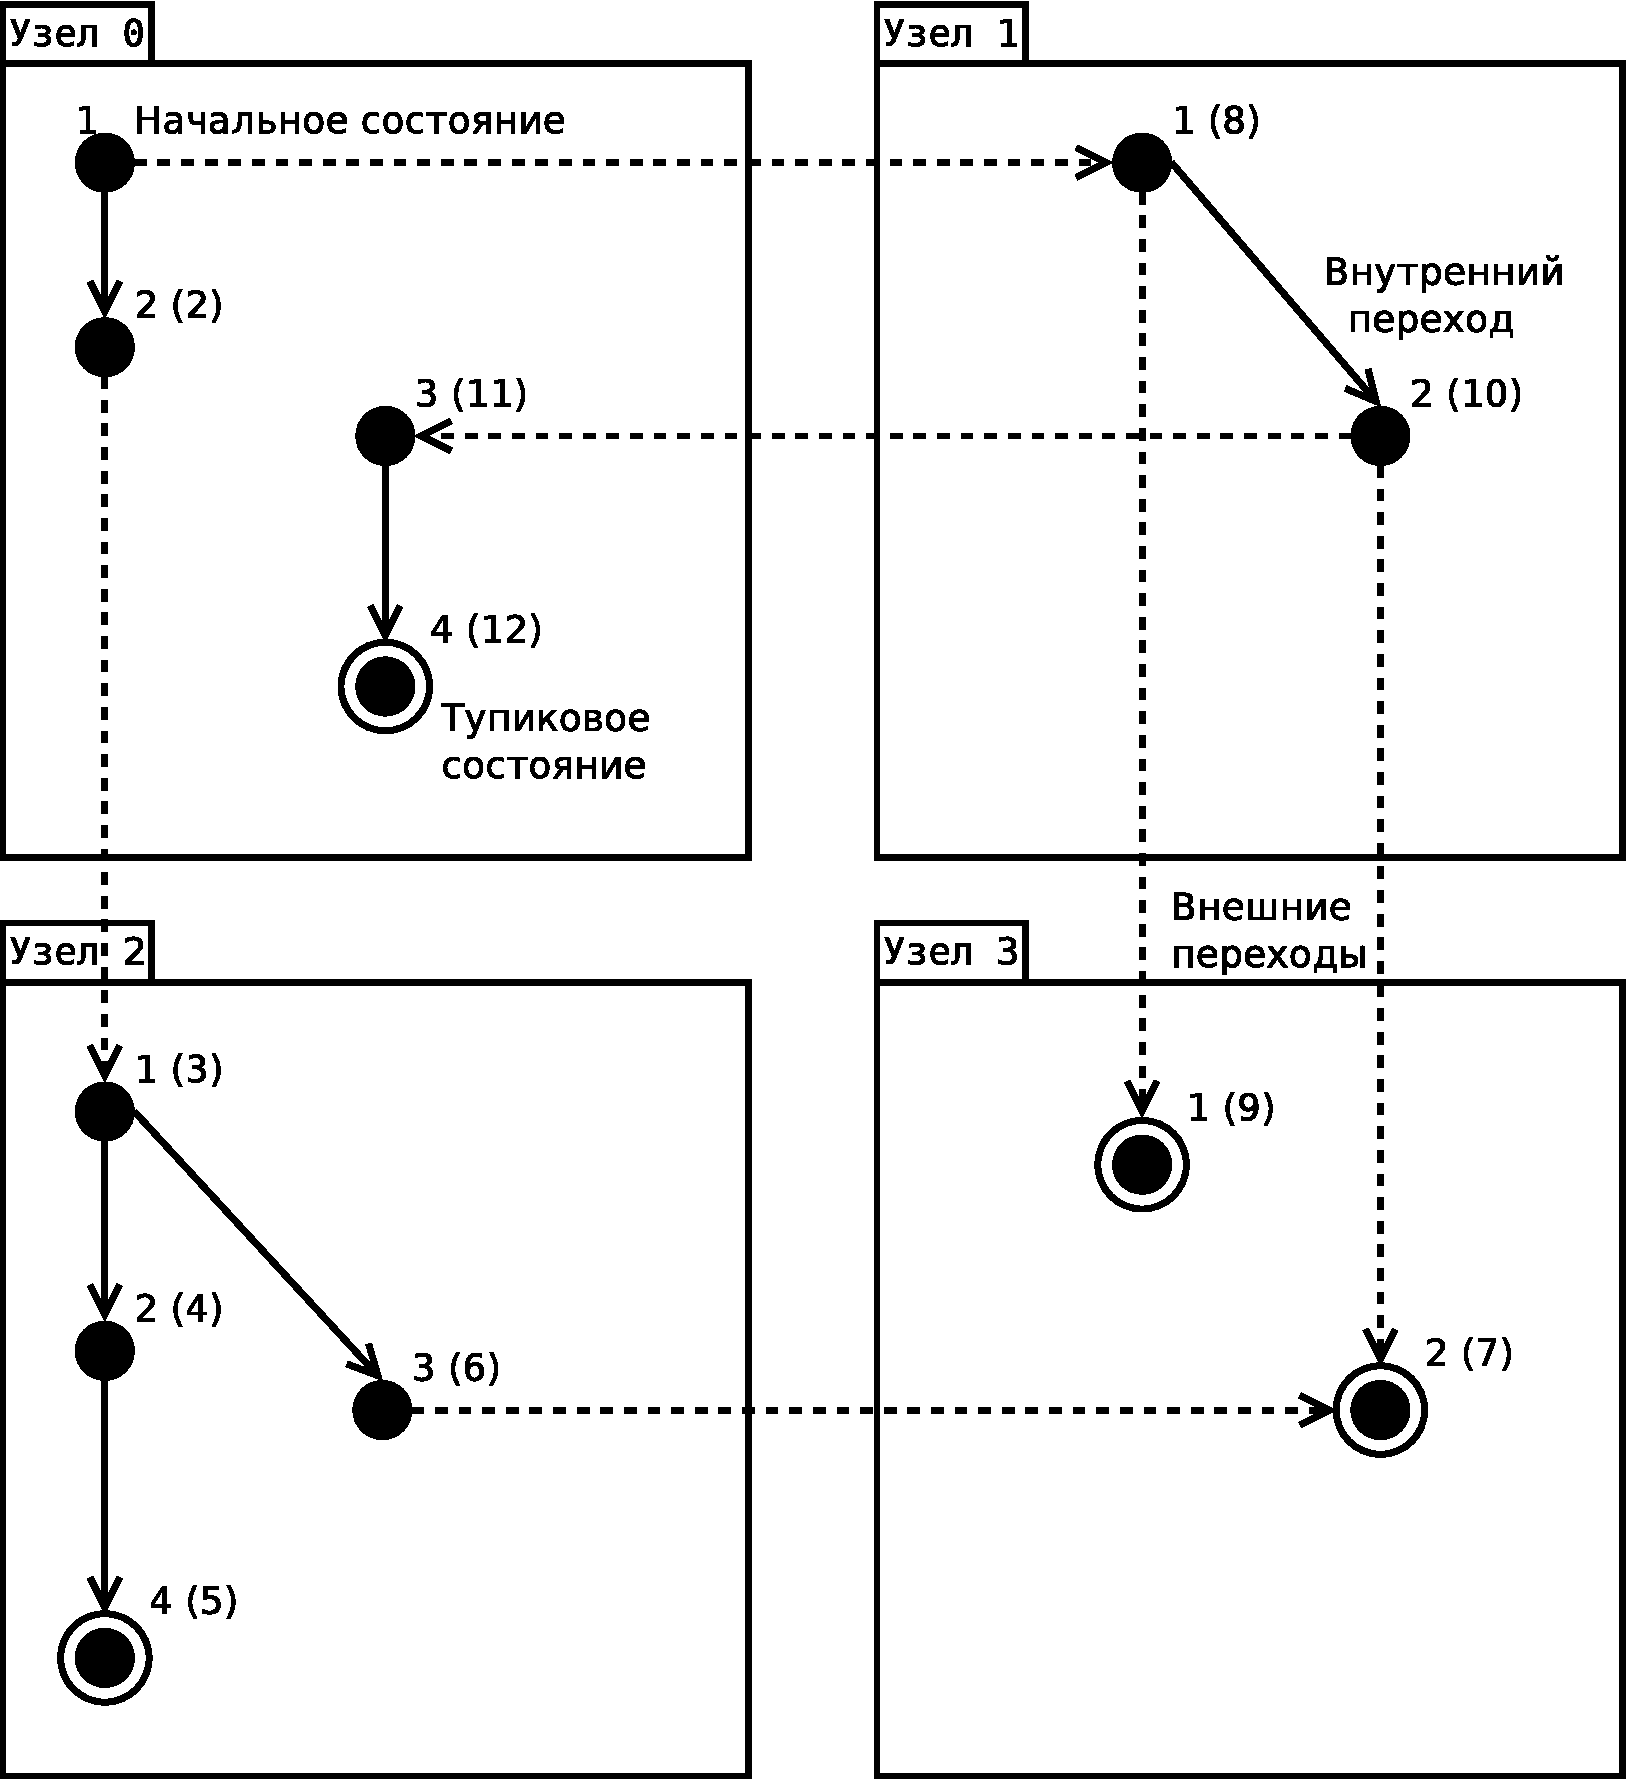
\includegraphics[width=0.6\textwidth]{graphics/distr-generation-2.pdf}
  \caption{.~Пример работы параллельной генерации состояний}
  \label{fig:distr-generation}
\end{figure}

Несмотря на очевидные преимущества, второй подход имеет свой недостаток: отсутствие какого-либо глобального порядка обхода состояний. В работе была выбрана параллельная генерации состояний. Каждый узел, кроме генерации состояний, также проверяет утверждения.

\section{Функция распределения состояний между узлами}
\label{sec:state-partition}

Одной из основных проблем параллельной генерации состояний является выбор функции распределения состояний между
узлами.
Эта функция ставит в соответствие каждому состоянию индекс узла, отвечающего за хранение данного
состояний.
В случае параллельной генерации состояний она должна иметь следующие свойства:

\begin{itemize}
\item зависеть только от битового представления самого состояния, поскольку одно и то же состояние
  может генерироваться различными узлами в результате различных переходов;

\item распределять состояния между узлами достаточно равномерно, в противном случае часть памяти у некоторых
  узлов будет простаивать;

\item обладать свойством локальности относительно переходов между состояниями~--- по возможности новые
  состояния должны принадлежать тому же узлу, что и исходное.
\end{itemize}

Наиболее простым подходом является использование хэш-функции от битового представление состояния $s$ в качестве индекса
хранящего его узла.
Это обеспечит первые два условия: если выбрана подходящая хэш-функция, распределение будет
достаточно равномерным.
Однако, третье условие при этом не соблюдается, поскольку все новые состояния имеют равные шансы
принадлежать любому узлу независимо того, на каком узле они были сгенерированы.

Пусть число узлов~--- $N$, состояний~--- $S$, переходов между ними~--- $T$.
В случае равномерного распределения состояний между узлами вероятность того, что следующее состояние будет принадлежать текущему узлу, равняется $1/N$.
Следовательно, вероятность того, что потребуется удаленный вызов, равна $1 - 1/N$, а среднее число удаленных
вызовов в течение всей генерации составит
\[\label{eq:rpc-partfull}
  Q = T (1 - \frac{1}{N}),
\]
что при больших значениях стремится к $T$.

Высокое число удаленных вызовов негативно отражаются на производительности, поэтому необходимо найти более удачную
функцию распределения состояний, которая бы удовлетворяла условию локальности.
Одна из возможных идей заключается в использовании хэш-код не от всего состояния $s$, а от некоторой его части $\tilde{s}$.

Битовое представление состояния в общем случае представляет собой набор значений переменных, описывающих состояние отдельных компонент моделируемой системы и значения общих переменных, описывающих взаимодействие между ними.

Пусть $P$~--- число таких компонент (процессов в нотации Promela) в модели, $k$~--- среднее число компонент, состояние которых меняется при переходе. Для языка Promela $1 \approx k < 2$ , поскольку взаимодействие между более чем двумя процессами (компонентами моделируемой системы) нереализуемо, но для двух процессов есть возможность синхронной передачи сообщения, при которой оба меняют свое состояние.
Последняя возможность используется обычно редко, поэтому для большинства моделей $k$ достаточно близко к 1.

Таким образом, битовое представления состояния естественным образом разделяется на $(P+1)$ область, с учетом области глобальных переменных.
При этом $P$ из них меняются почти независимо друг от друга при условии $k \approx 1$, и в качестве хэшируемого подсостояния $\tilde{s}$ можно выбрать первые (или произвольные) $\rho$ областей, хранящих локальные состояния первых $\rho$ процессов.

Если предположить, что каждый процесс $p_i$ участвует примерно в равной доле переходов, то для произвольного наперед заданного процесса вероятность участия в данном переходе составит $k/\rho$, а для $\rho$ процессов при $k \approx 1$ либо небольшом $\rho$~--- $\frac{k \rho}{P}$.
При условии, что множество возможных локальных состояний процесса отображается на множество узлов равномерным образом, вероятность удаленного вызова при изменении локального состояния процесса (т.е. при его участии в переходе), по аналогии с предыдущими рассуждениями, составит $1 - 1/N$. Количество удаленных вызовов во всей модели, таким образом, равняется
\[\label{eq:rpc-partproc}
  Q_\rho = \frac{k \rho}{P} T (1 - \frac{1}{N})
\]
и с ростом $N$ стремится к $\frac{k \rho}{P} T$. При количестве процессов $P = 10$, $k = 1.1$ и $\rho = 2$, число удаленных вызовов уменьшается примерно в 4 раза в сравнении с <<наивным>> подходом.

Выбор меньших значений $\rho$ приводит к меньшему числу удаленных вызовов, однако увеличивает неравномерность распределения, поэтому его значение следует выбирать из баланса между требуемой равномерностью распределения состояний и выигрышем во времени за счет уменьшения числа вызовов.

Пусть $i$-ый процесс $p_i$ имеет $w_i$ возможных значений локального состояний, т.е. число допустимых комбинаций значений его переменных составляет $w_i$.
Объединение локальных состояний $\rho$ процессов тогда имеет не более $W_\rho = \prod_{i=1}^{\rho}{w_i}$ возможных значений.
Число значений может быть меньше $W_\rho$, поскольку в общем случае не все комбинации являются допустимыми.
Значение $\rho$ должно обеспечивать условие $W_\rho \gg N$, иначе, особенно при $W_\rho \approx N$, распределение будет неравномерным даже при удачном выборе хэш-функции, а при $W_\rho < N$ память некоторых узлов не будет использоваться вообще, так как число возможных значений хэш-функции будем меньше числа узлов.

\section{Реализация экспериментальной системы}
\label{sec:implementation}

Было создано программное средство для параллельной проверки состояний с распределенной генерацией, поддерживающее основные возможности языка Promela для описания модели и проверку утверждений с функцией \textbf{assert} и поиском тупиковых состояний.

\begin{figure}[ht]
  \centering
  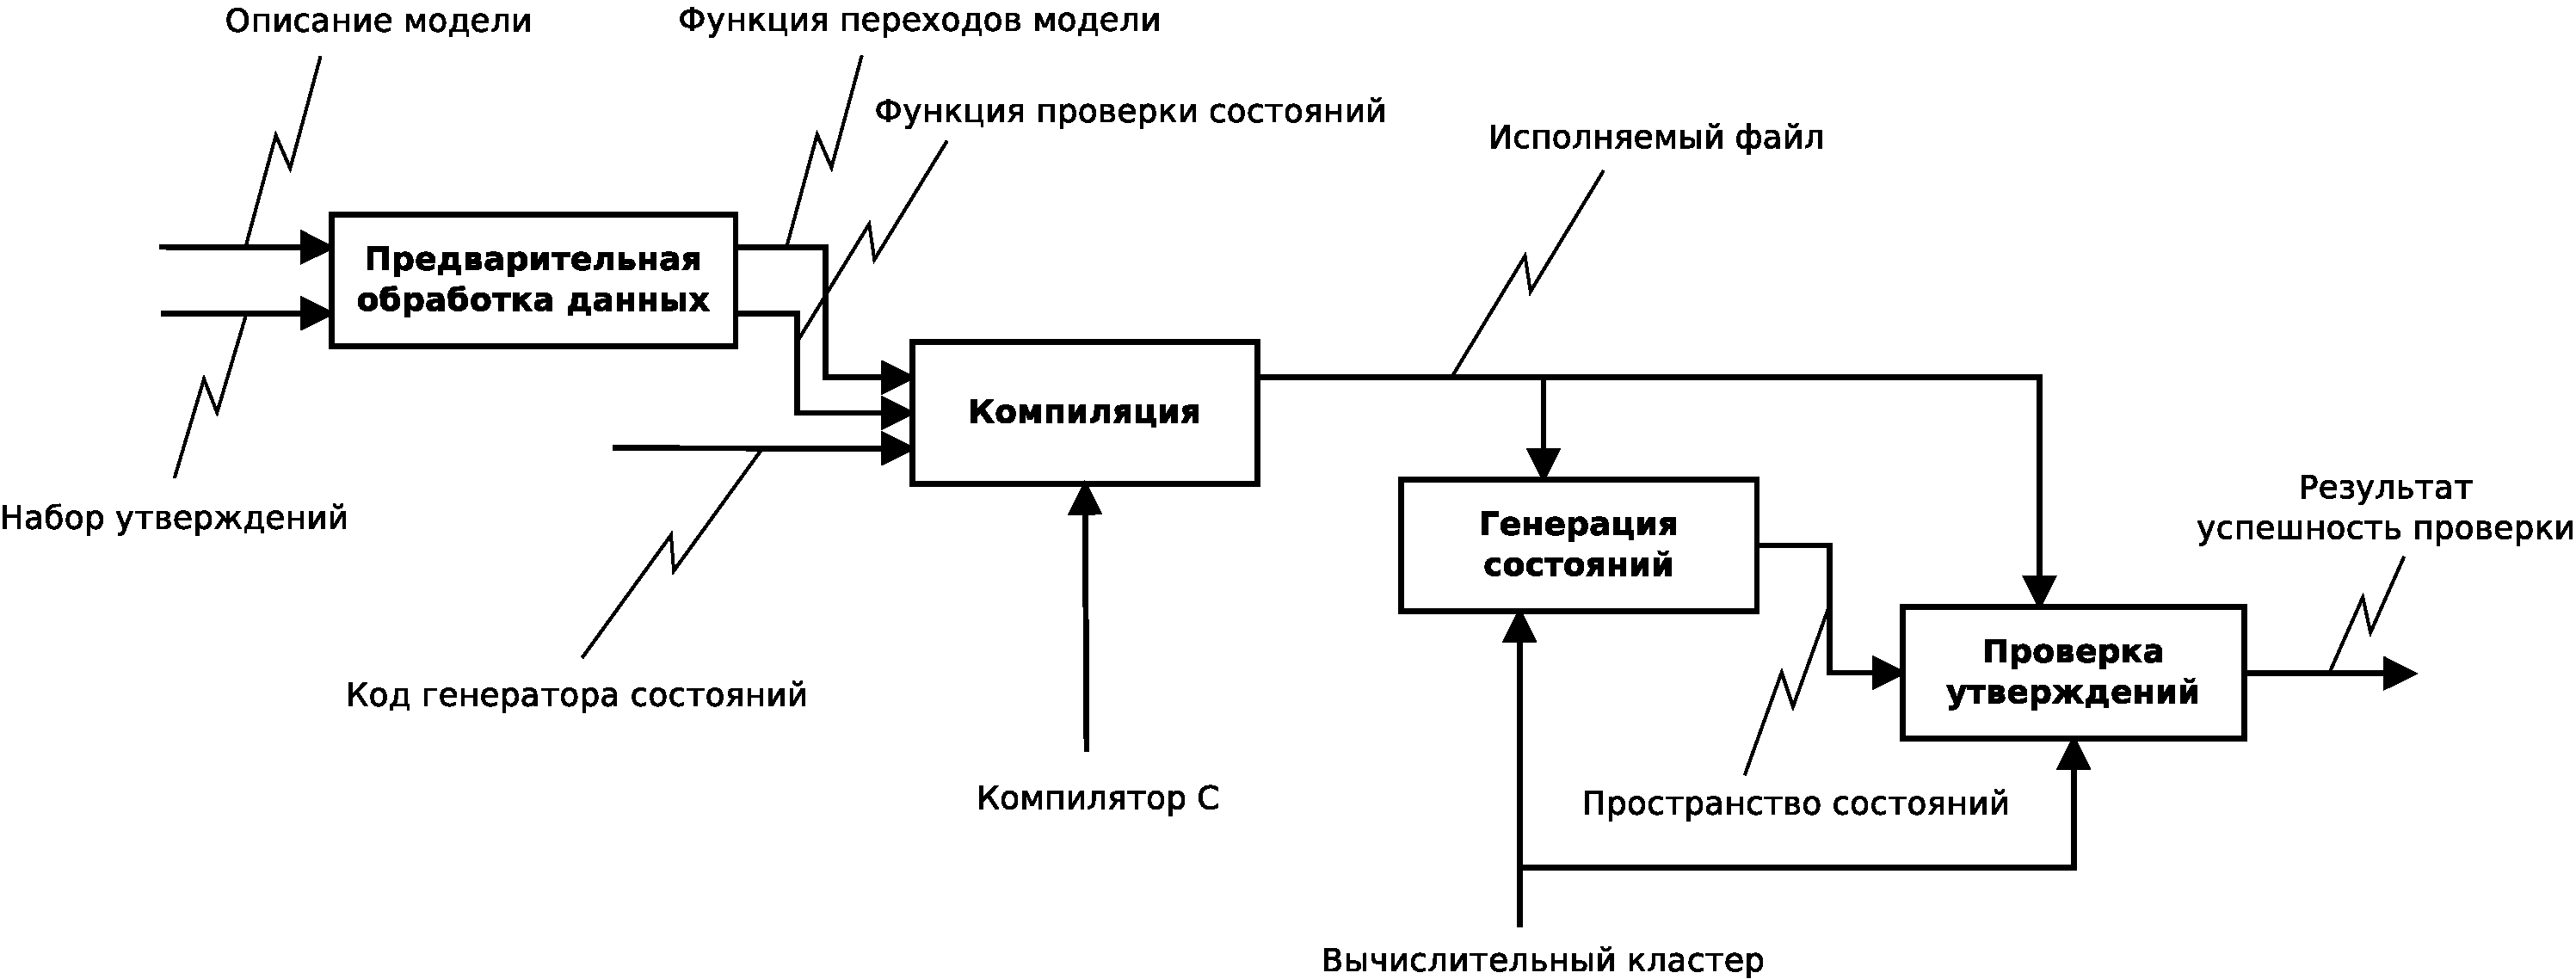
\includegraphics[width=\textwidth]{graphics/stategen-idef0-simple.pdf}
  \caption{.~Функциональная схема процесса генерации кода по описанию модели}
  \label{fig:stategen-idef0-simple}
\end{figure}

Разработанное ПО работает следующим образом (рис.~\ref{fig:stategen-idef0-simple}). Исходная модель на Promela считывается и транслируется во внутренний граф команд для каждого процесса, который затем минимизируется.
С целью достижения скорости генерации состояний, сравнимой со скоростью системы SPIN, по полученным графам команд генерируется код на языке~C, выполняющий вычисление функции переходов модели $Next(s) = \{s': R(s, s')\}$ и функции проверки состояний $Assert(s): S \rightarrow \{0, 1\}$.
В качестве платформы для параллельных вычислений в системе используется вычислительный кластер, поддерживающий стандарт MPI.

\section{Результаты экспериментов}
\label{sec:experim}

В качестве исходных данных для экспериментов были взяты две модели: выбора лидера и <<обедающие философы>> с числом компонент $P = 6$.
Для проведения экспериментов использовался MPI-кластер из 20 узлов, имеющих 4 Гб ОЗУ и 4 ЦПУ Intel\,Xeon\,5120~1.86 ГГц каждый.


Результаты экспериментов по сравнению предлагаемого распределения с $\rho = 1$ и $\rho = 2$ с наивным представлены на табл.~\ref{tab:election-results} и~\ref{tab:philo-results}.

\begin{table}[htb]
  \centering
  \begin{tabular}{|c|c|c|c|c|}
    \hline
    $\rho$ & Доля внешних        & Неравномерность   & Время простоя, & Общее время \\
           & переходов, \%       & распределения, \% & сек            & работы, сек                 \\ \hline
    1      & 16                  & \textbf{66.3}     & 29             & 43                  \\ \hline
    2      & 36                  & 12.8              & 65             & 84                  \\ \hline
    ---    & \textbf{87}         & 0.1               & \textbf{127}   & \textbf{164}        \\ \hline
  \end{tabular}
  \caption{.~Сравнение распределений (алгоритм выбора лидера)}
  \label{tab:election-results}
\end{table}

\begin{table}[htb]
  \centering
  \begin{tabular}{|c|c|c|c|c|}
    \hline
    $\rho$ & Доля внешних        & Неравномерность   & Время простоя, & Общее время \\
           & переходов, \%       & распределения, \% & сек            & работы, сек         \\ \hline
    1      & 17                  & \textbf{89.4}     & 3              & 14                  \\ \hline
    2      & 35                  & 29.6              & 7              & 21                  \\ \hline
    ---    & \textbf{88}         & 0.1               & \textbf{50}    & \textbf{75}         \\ \hline
  \end{tabular}
  \caption{.~Сравнение распределений (<<обедающие философы>>)}
  \label{tab:philo-results}
\end{table}


Проблемные значения выделены жирным начертанием. В таблицах приведены следующие величины:

\begin{itemize}
\item доля внешних переходов~--- отношение числа удаленных вызовов (суммарно на всех узлах) к числу переходов $T$;
\item неравномерность распределения~--- отношение среднеквадратичного отклонения к среднему для последовательности $m_1
  m_2 \ldots m_N$, где $m_i$~--- число состояний, хранимых узлом $i$;
\item время простоя при ожидании сообщений от других узлов (сетевые задержки);
\item общее время работы.
\end{itemize}

Из приведённых результатов можно сделать следующие выводы.

\begin{enumerate}
\item Выбор распределения между узлами важен, поскольку время простоя за счет удаленных вызовов составляет существенного
  часть от времени выполнения.

\item При <<наивном>> подходе к распределению состояний число удаленных вызовов близко к числу всех переходов, как и следует из~(\ref{eq:rpc-partfull}).

\item Предлагаемый способ распределения состояний по первым $\rho$ процессам позволяет уменьшить число удаленных вызовов
  и время выполнения по сравнению с <<наивным>> подходом в соответствии с~(\ref{eq:rpc-partproc}).

\item Необходим подбор параметра $\rho$ в соответствии со свойствами проверямой модели ($P, w_i$) для обеспечения
  требуемого уровня равномерности распределения состояний; в частности, значения $\rho = 1$ в приведенных экспериментах
  оказалось недостаточно, поскольку неравномерность до 90\% означает, что большая часть памяти некоторых узлов не
  используется вообще.
\end{enumerate}

\section-{Заключение}

Предложена функция разбиения пространства состояний, позволяющая уменьшить число удаленных вызовов между узлами при сохранении равномерности распределения.
Эксперименты, проведенные при помощи прототипа средства параллельной проверки моделей, показывают, что предложенное разбиение в несколько раз сокращает время проверки в сравнении с тривиальным.
Полученный алгоритм можно использовать для параллельной проверки моделей большего размера, чем позволяют традиционные последовательные подходы.

\begin{thebibliography}{9}

\bibitem{Clarke}
\textit{Э. М. Кларк, О. Грамберг, Д. Пелед}. Верификация моделей программ. Москва: МЦНМО, 2002. 416~c.

\bibitem{BitHash1}
\textit{Holzmann, G. J.} An Analysis of Bitstate Hashing // Formal Methods in System Design. 1998. Vol. 13, N. 3. Pp. 287–305.

\bibitem{SPIN}
\textit{Holzmann, G. J.} The model checker SPIN  // IEEE Transactions on Software Engineering. 1997. Vol. 23. Pp. 279–295.

\end{thebibliography}

\end{document}

